\chapter{Notes}

Just a collection of random notes about possible findings/decisions. Will later be converted into actual content.

\section{GitHub Crawling}

Different approaches:\\
web ui vs api\\
The web ui is built on the api and can be used with the same query parameters as the api. On top of that the web ui has the same limitations as the api, except possible rate-limiting. Further on the api will be used as it allows to query quicker and with less overhead.\\

directly search for filename\\
search for filename in the description or readme of any repository\\

current limitations:\\
Per search query a maximum result of 1000 entries can be returned.\\
Meaning a naive search for docker-compose would result in a total\_count of 800k results of which you can only view 1000.\\

Ways to mitigate that:\\
GitHub offers various kinds of query parameters\\
<<possible list some and explain>>\\
Querying the api allows only the following parameters, where q is further divided into extra "parameters":\\
q=\{extension\\
file size\\
path\\
file name\}\\
sort\\
order\\
page\\
\\
to get unique urls and to be able to search for more than just 1000 files, we will utilize the size parameter, which allows values of either Integer or Integer..Integer, meaning a range. The values supplied will be interpreted by GitHub as bytes. Therefore we can search for more files as on a byte level files are more likely to be distributed as not all share the same size due to obvious reasons (content). <<refer to how docker-compose files are structured>>

\section{Database}
The aim is to build a knowledge graph or graph in general to be able to utilize it further for either recommender systems or proper analysis of relations between the usage of images.

Comparisson between possible Databases?\\

Neo4j\\
- proper Graph Database\\
- querying feels super outdated\\
- only directed edges\\
- node.js support\\

Grakn.ai\\
- underlying system is a Graph, but more knowledge orientated\\
- designed for machines (output/input)\\
- hypergraph\\
- node.js support\\
\\
Currently in favour of grakn.\\
Next step: define Modell\\
\subsection{Entity–relationship model}
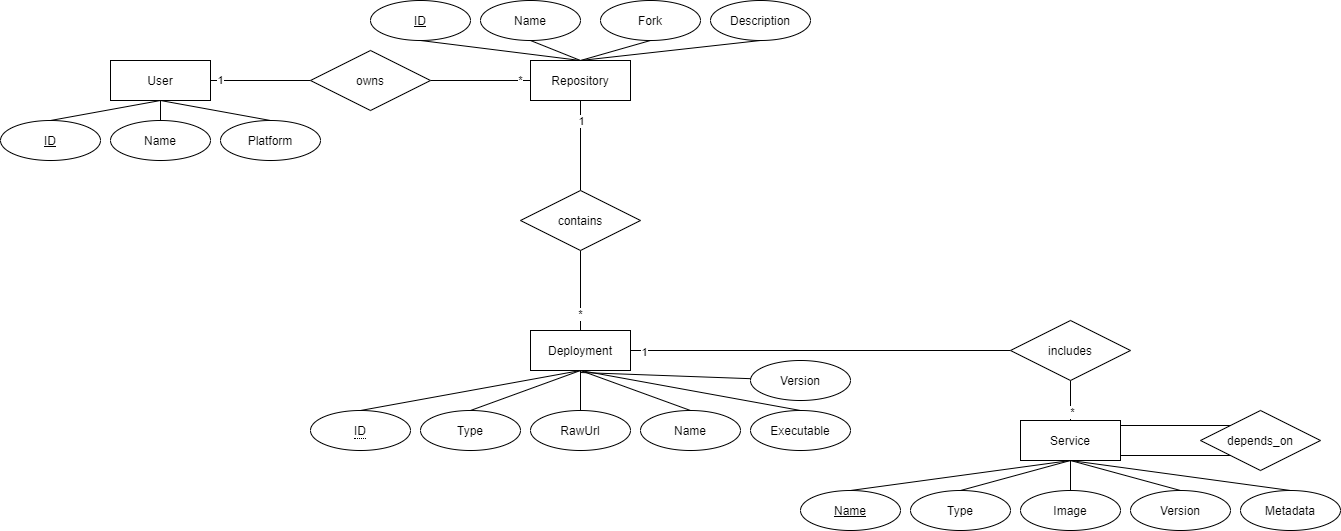
\includegraphics[width=1.2\paperwidth,height=1.2\paperheight,keepaspectratio,angle=270]{graphics/er_database.png}